\let\negmedspace\undefined
\let\negthickspace\undefined
\documentclass[journal]{IEEEtran}
\usepackage[a5paper, margin=10mm, onecolumn]{geometry}
%\usepackage{lmodern} % Ensure lmodern is loaded for pdflatex
\usepackage{tfrupee} % Include tfrupee package

\setlength{\headheight}{1cm} % Set the height of the header box
\setlength{\headsep}{0mm}     % Set the distance between the header box and the top of the text

\usepackage{gvv-book}
\usepackage{gvv}
\usepackage{cite}
\usepackage{amsmath,amssymb,amsfonts,amsthm}
\usepackage{algorithmic}
\usepackage{graphicx}
\usepackage{textcomp}
\usepackage{xcolor}
\usepackage{txfonts}
\usepackage{listings}
\usepackage{enumitem}
\usepackage{mathtools}
\usepackage{gensymb}
\usepackage{comment}
\usepackage[breaklinks=true]{hyperref}
\usepackage{tkz-euclide} 
\usepackage{listings}
% \usepackage{gvv}                                        
\def\inputGnumericTable{}                                 
\usepackage[latin1]{inputenc}                                
\usepackage{color}                                            
\usepackage{array}                                            
\usepackage{longtable}                                       
\usepackage{calc}                                             
\usepackage{multirow}                                         
\usepackage{hhline}                                           
\usepackage{ifthen}                                           
\usepackage{lscape}
\begin{document}

\bibliographystyle{IEEEtran}
\vspace{3cm}
\title{1.9.16}
\author{EE24BTECH11008 - Aslin Garvasis
}
% \maketitle
% \newpage
% \bigskip
{\let\newpage\relax\maketitle}

\renewcommand{\thefigure}{\theenumi}
\renewcommand{\thetable}{\theenumi}
\setlength{\intextsep}{10pt} % Space between text and floats


\numberwithin{equation}{enumi}
\numberwithin{figure}{enumi}
\renewcommand{\thetable}{\theenumi}
 \textbf{Question:}\\Find the distance between the points $\brak{a,b}$ and $\brak{-a,-b}$ 
 
 \solution 
 \begin{table}[h!]    
  \centering
  \begin{tabular}[12pt]{ |c| c|}
    \hline
	\textbf{Variable}  & \textbf{Description} \\
    \hline
	$\vec{A}$$\brak{a,b}=\brak{8,9}$ &  coordinates of first point\\
    \hline 
	$\vec{B}$$\brak{-a,-b}=\brak{-8,-9}$ & coordinates of second point\\
    \hline
	$\vec{\brak{A-B}^T}\vec{\brak{A-B}}=\norm{\vec A-\vec B }^2$ &square of distance between $\vec A$ and $\vec B$\\  
    \hline
	$d$ & distance between $\vec A$ and $\vec B$\\
    \hline 	
         
\end{tabular}

  \caption{Input parameters}
  \label{tab1.1.9.16}
\end{table}
\begin{align}
\implies d&=\norm{ \vec A-\vec B}=\sqrt{\vec{\brak{A-B}}^T\vec{\brak{A-B}}}\\ 
	\implies d&=\sqrt{\myvec{2a&2b}\myvec{2a\\2b}}\\
	\implies d&=\sqrt{4a^2+4b^2}\\ 
	\implies d&=2\sqrt{a^2+b^2}\\
	\implies d&=2\sqrt{145}
\end{align}
\begin{figure}[h!]
                \centering
               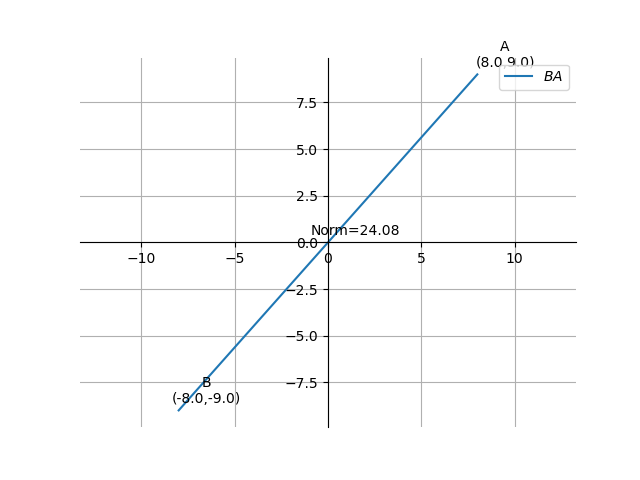
\includegraphics[width=0.7\linewidth]{Figs/Fig1.png}
               \label{stemplot}
               \end{figure}
\end{document}
